\documentclass[10pt,a4paper]{article}  % Déclare la classe du document.

\newcommand{\chaptermark}[2]{\og #2 \fg{} (#1)} % ligne uniquement pour éviter une erreur en cas d'article
\usepackage[table,dvipsnames,svgnames]{xcolor}
\usepackage{listingsutf8}
%\usepackage[utf8]{inputenc}% gestion des accents (source)
\usepackage[T1]{fontenc}% gestion des accents (PDF)
\usepackage{fontspec}
\usepackage[french]{babel}% gestion du français
\usepackage{textcomp}% caractères additionnels
\usepackage{mathtools,amssymb,amsthm}% packages de l'AMS + mathtools
\usepackage{amsmath}
\usepackage{yhmath}
\usepackage{mathpazo}
\usepackage[scaled=0.95]{helvet}
\usepackage{courier}
%\usepackage{fourier}
%\usepackage[scaled=0.95]{helvet}
%\usepackage{courier}
\usepackage{bm}
\usepackage{gensymb}
\usepackage{graphicx}

\usepackage{enumitem}
\usepackage{pifont}

\usepackage{pstricks}
\usepackage{pstricks-add}
\usepackage{pst-eucl}
\usepackage{pgfplots}
\let\clipbox\relax
%\usepackage{pst-plot,pst-text,pst-tree,pstricks-add}
%\usepackage{pst-node} % required package
\usepackage{pst-all}
\usepackage[most,skins,breakable]{tcolorbox}

\usepackage{euscript}





% ############### Nouvelles commandes ###############
% Coloration des labels des points dans pst-eucl
\makeatletter
\define@key[psset]{pst-eucl}{LabelColor}{\def\psk@LabelColor{#1}}
\psset{LabelColor=black}
\def\Pst@WhichLabel#1{{\color{\psk@LabelColor}%
		\ifx\psk@PointName\@default#1\else\psk@PointName\fi}}
\makeatother

% renomme le symbole #2 en #1#2 et invalide le symbole initial #2:
\def\renamesymbol#1#2{
	\expandafter\let\expandafter\newsym\expandafter=\csname#2\endcsname
	\expandafter\global\expandafter\let\csname#1#2\endcsname=\newsym
	\expandafter\global\expandafter\let\csname#2\endcsname=\origsym
}



\usepackage{ProfCollege}
\renamesymbol{Casio}{Calculatrice}
\usepackage[nonshellescape]{ProfLycee}



%\usepackage[left=1.5cm,right=1.5cm,top=2.5cm,bottom=2.5cm]{geometry}
\usepackage[left=13mm,right=13mm,top=18mm,bottom=18mm,footskip=30pt]{geometry}
\setlength{\headheight}{15pt}

\usepackage{titlesec}
\usepackage{pas-math}
\usepackage{longtable}
\usepackage{tikz,tkz-tab}
\usepackage{amsmath}
\usepackage[right]{eurosym}
\usepackage{sectsty}
\usepackage{tipfr}
\usepackage{setspace}

%pour faire les touches de la calculatrices
\usepackage{menukeys}
\renewmenumacro{\menu}{roundedmenus} % default: menus
\renewmenumacro{\directory}{pathswithfolder} % default: paths
\renewmenumacro{\keys}{shadowedroundedkeys} % default: roundedkeys


\usepackage{multicol}
\usepackage{multirow}
\usepackage{systeme}

%% Format des titres de chapitres, paragraphes, ...
\titleformat{\chapter}[frame]
{\color{red!85!white}\normalsize}%
{\filright\sffamily\Large%
	\enspace Chapitre \thechapter\enspace}%
{8pt}
{\color{red!85!white}\rule{0pt}{30pt}\sffamily\Huge\bfseries\filcenter}
%%%%%%%%%%%%%%%%%%%%
\titlespacing{\chapter}{0pc}{0pc}{2pc}
\titlespacing{\subsection}{2pc}{}{}

\titleformat{\subsection}[block]{\hspace{1em}}{\thesubsection}{1em .}{}
\titleformat{\subsubsection}[block]{\hspace{2em}}{\thesubsection}{1em )}{}

\chapterfont{\color{red}{}}
\sectionfont{\color{green!55!black}{}}
\subsectionfont{\color{cyan!65!black}{}}
\subsubsectionfont{\color{violet}{}}
\renewcommand{\thesection}{\color{green!55!black}\Roman{section}.}
\renewcommand{\thesubsection}{\color{cyan!65!black}\arabic{subsection})}
\renewcommand{\thesubsubsection}{\color{violet}\alph{subsubsection})}
\setcounter{secnumdepth}{3}

\titleformat{\subsection}[block]{\hspace{1em}}{\thesubsection}{1em .}{}
\titleformat{\subsubsection}[block]{\hspace{2em}}{\thesubsection}{1em )}{}

\usepackage[column=A]{cellspace}
\setlength{\cellspacebottomlimit}{4pt}
\setlength{\cellspacetoplimit}{4pt}
\setlength{\parindent}{2pt}
\setlength{\tabcolsep}{0.5cm}


%entête et pieds de pages
\usepackage{fancyhdr}
\pagestyle{fancy}
\fancyhf{}
\usepackage{lastpage}
\renewcommand{\chaptermark}[1]{\markboth {Chap. \thechapter~ - ~#1}{}}
\renewcommand\headrulewidth{1pt}
\fancyhead[LO,RE]{1ère G - spécialité maths}
\fancyhead[RO,LE]{\leftmark}
\renewcommand\footrulewidth{1pt}
\fancyfoot[LO,RE]{Année 2025-2026}
\fancyfoot[RO,LE]{\textbf{Page \thepage/\pageref{LastPage}}}

%Mes boites pour les définitions, propriétés, remarques, ...

%Mes boites pour les définitions, propriétés, remarques, ...

\newcommand\titrebox[1]{\textbf{#1}}
\newtcolorbox{definition}{breakable,colback=red!10!white,
	colframe=red!85!white, fonttitle=\bfseries,enhanced,
	attach boxed title to top left={xshift=5mm, yshift=-2mm},boxed title style={size=small,colback=red!10!white,colframe=red!85!white, arc=0.5mm},
	title=\textcolor{red!85!white}{Définition} , arc=3mm}

\newtcolorbox{definitionTitre}[1]{breakable,colback=red!10!white,
	colframe=red!85!white, fonttitle=\bfseries,enhanced,
	attach boxed title to top left={xshift=5mm, yshift=-2mm},boxed title style={size=small,colback=red!10!white,colframe=red!85!white, arc=0.5mm},
	title=\textcolor{red!85!white}{Définition - #1} , arc=3mm}

\newtcolorbox{definitionPerso}[1]{breakable,colback=red!10!white,
	colframe=red!85!white, fonttitle=\bfseries,enhanced,
	attach boxed title to top left={xshift=5mm, yshift=-2mm},boxed title style={size=small,colback=red!10!white,colframe=red!85!white, arc=0.5mm},
	title=\textcolor{red!85!white}{#1} , arc=3mm}

\newtcolorbox{regle}{breakable,colback=red!10!white,
	colframe=red!85!white, fonttitle=\bfseries,enhanced,
	attach boxed title to top left={xshift=5mm, yshift=-2mm},boxed title style={size=small,colback=red!10!white,colframe=red!85!white, arc=0.5mm},
	title=\textcolor{red!85!white}{Règle} , arc=3mm}

\newtcolorbox{regles}{breakable,colback=red!10!white,
	colframe=red!85!white, fonttitle=\bfseries,enhanced,
	attach boxed title to top left={xshift=5mm, yshift=-2mm},boxed title style={size=small,colback=red!10!white,colframe=red!85!white, arc=0.5mm},
	title=\textcolor{red!85!white}{Règles} , arc=3mm}

\newtcolorbox{definitions}{breakable,colback=red!10!white,
	colframe=red!85!white, fonttitle=\bfseries,enhanced,
	attach boxed title to top left={xshift=5mm, yshift=-2mm},boxed title style={size=small,colback=red!10!white,colframe=red!85!white, arc=0.5mm},
	title=\textcolor{red!85!white}{Définitions} , arc=3mm}

\newtcolorbox{propriete}{breakable,colback=red!10!white,
	colframe=red!85!white, fonttitle=\bfseries,enhanced,
	attach boxed title to top left={xshift=5mm, yshift=-2mm},boxed title style={size=small,colback=red!10!white,colframe=red!85!white, arc=0.5mm},
	title=\textcolor{red!85!white}{Propriété} , arc=3mm}

\newtcolorbox{proprieteTitre}[1]{breakable,colback=red!10!white,
	colframe=red!85!white, fonttitle=\bfseries,enhanced,
	attach boxed title to top left={xshift=5mm, yshift=-2mm},boxed title style={size=small,colback=red!10!white,colframe=red!85!white, arc=0.5mm},
	title=\textcolor{red!85!white}{Propriété - #1} , arc=3mm}

\newtcolorbox{proprietes}{breakable,colback=red!10!white,
	colframe=red!85!white, fonttitle=\bfseries,enhanced,
	attach boxed title to top left={xshift=5mm, yshift=-2mm},boxed title style={size=small,colback=red!10!white,colframe=red!85!white, arc=0.5mm},
	title=\textcolor{red!85!white}{Propriétés} , arc=3mm}

\newtcolorbox{theoreme}{breakable,colback=red!10!white,
	colframe=red!85!white, fonttitle=\bfseries,enhanced,
	attach boxed title to top left={xshift=5mm, yshift=-2mm},boxed title style={size=small,colback=red!10!white,colframe=red!85!white, arc=0.5mm},
	title=\textcolor{red!85!white}{Théorème} , arc=3mm}

\newtcolorbox{theoremeTitre}[1]{breakable,colback=red!10!white,
	colframe=red!85!white, fonttitle=\bfseries,enhanced,
	attach boxed title to top left={xshift=5mm, yshift=-2mm},boxed title style={size=small,colback=red!10!white,colframe=red!85!white, arc=0.5mm},
	title=\textcolor{red!85!white}{Théorème - #1} , arc=3mm}

\newtcolorbox{theoremes}{breakable,colback=red!10!white,
	colframe=red!85!white, fonttitle=\bfseries,enhanced,
	attach boxed title to top left={xshift=5mm, yshift=-2mm},boxed title style={size=small,colback=red!10!white,colframe=red!85!white, arc=0.5mm},
	title=\textcolor{red!85!white}{Théorèmes} , arc=3mm}

\newtcolorbox{bexemple}{
	enhanced,
	breakable,
	fonttitle=\bfseries,
	frame empty,
	nobeforeafter,
	borderline west={0.5mm}{0mm}{cyan!75!black},
	title=\textcolor{cyan!75!black}{\faHubspot\:\:Exemple},
	%title after break=Exemple (suite),
	colback=white,
	extras={enhanced, frame empty},
	detach title,before upper={\tcbtitle\ :\quad },
}

\newtcolorbox{bexemples}{
	enhanced,
	breakable,
	fonttitle=\bfseries,
	frame empty,
	nobeforeafter,
	borderline west={0.5mm}{0mm}{cyan!75!black},
	title=\textcolor{cyan!75!black}{\faHubspot\:\:Exemples},
	%title after break=Exemples (suite),
	colback=white,
	extras={enhanced, frame empty},
	detach title,before upper={\tcbtitle\ :\quad },
}

\newtcolorbox{bexemplet}[1]{
	enhanced,
	breakable,
	fonttitle=\bfseries,
	frame empty,
	borderline west={0.5mm}{0mm}{cyan!75!black},
	title=\textcolor{cyan!75!black}{\faHubspot\:\:Exemple - #1},
	colback=white,
	extras={enhanced, frame empty},
	detach title,before upper={\tcbtitle\ :\quad },
}

\newtcolorbox{brmq}{
	enhanced,
	breakable,
	fonttitle=\bfseries,
	frame empty,
	nobeforeafter,
	borderline west={0.5mm}{0mm}{orange!95!white},
	title=\textcolor{orange!85!white}{\faHandPointRight[regular]\:\:Remarque} ,
	colback=white,
	extras={enhanced, frame empty},
	detach title,before upper={\tcbtitle\ \quad },
}

\newtcolorbox{brmqs}{
	enhanced,
	breakable,
	fonttitle=\bfseries,
	frame empty,
	nobeforeafter,
	borderline west={0.5mm}{0mm}{orange!85!white},
	title=\textcolor{orange!85!white}{\faHandPointRight[regular]\:\:Remarques},
	colback=white,
	detach title,before upper={\tcbtitle\ \quad },
	extras={enhanced, frame empty},
}

\newtcolorbox{brmqt}[1]{
	enhanced,
	breakable,
	fonttitle=\bfseries,
	frame empty,
	nobeforeafter,
	borderline west={0.5mm}{0mm}{orange!85!white},
	title=\textcolor{orange!85!white}{\faHandPointRight[regular]\:\:Remarque - #1},
	colback=white,
	extras={enhanced, frame empty},
	detach title,before upper={\tcbtitle\ \quad },
}

\newtcolorbox{consequences}[1]{
	enhanced,
	breakable,
	fonttitle=\bfseries,
	frame empty,
	nobeforeafter,
	borderline west={0.5mm}{0mm}{ProcessBlue},
	title=\textcolor{ProcessBlue}{#1},
	colback=white,
	extras={enhanced, frame empty},
	detach title,before upper={\tcbtitle\ :\quad },
}

\newtcolorbox{bmethode}{
	enhanced,
	breakable,
	fonttitle=\bfseries,
	frame empty,
	nobeforeafter,
	borderline west={0.5mm}{0mm}{blue!75!black},
	title=\textcolor{blue!75!black}{Méthode} ,
	colback=white,
	extras={enhanced, frame empty},
	attach boxed title to top left = {xshift = -3mm},
	boxed title style={size=small,colback=white,colframe=blue!75!black, arc=3mm,
	}
}

\newtcolorbox{bmethodes}{
	enhanced,
	breakable,
	fonttitle=\bfseries,
	frame empty,
	nobeforeafter,
	borderline west={0.5mm}{0mm}{blue!75!black},
	title=\textcolor{blue!75!black}{Méthodes} ,
	colback=white,
	extras={enhanced, frame empty},
	attach boxed title to top left = {xshift = -3mm},
	boxed title style={size=small,colback=blue!75!black,colframe=blue!75!black, arc=3mm,
	}
	boxed title after break style={size=small,colback=white,colframe=blue!75!black, arc=3mm,
	}
}

\newtcolorbox{bmethodet}[1]{
	enhanced,
	breakable,
	fonttitle=\bfseries,
	frame empty,
	nobeforeafter,
	borderline west={0.5mm}{0mm}{blue!75!black},
	title=\textcolor{blue!75!black}{\faTasks\:\:Méthode - #1} ,
	colback=white,
	extras={enhanced, frame empty},
	attach boxed title to top left = {xshift = -3mm},
	boxed title style={size=small,colback=white,colframe=blue!75!black, arc=3mm,
	}
}

\newtcolorbox{bdemo}{
	enhanced,
	breakable,
	fonttitle=\bfseries,
	frame empty,
	nobeforeafter,
	borderline west={0.5mm}{0mm}{violet!65!white},
	title={\faEdit[regular]\:\:Démonstration},
	%title after break=Démonstration (suite),
	colback=white,
	extras={enhanced, frame empty},
	attach boxed title to top left = {xshift = -3mm},
	boxed title style={size=small,colback=violet!65!white,colframe=violet!65!white, arc=3mm,
	}
}

\newtcolorbox{bdemos}{
	enhanced,
	breakable,
	fonttitle=\bfseries,
	frame empty,
	nobeforeafter,
	borderline west={0.5mm}{0mm}{violet!65!white},
	title={\faEdit[regular]\:\:Démonstrations},
	%title after break=Démonstration (suite),
	colback=white,
	extras={enhanced, frame empty},
	attach boxed title to top left = {xshift = -3mm},
	boxed title style={size=small,colback=violet!65!white,colframe=violet!65!white, arc=3mm,
	}
}

\newtcolorbox{bdemot}[1]{
	enhanced,
	breakable,
	fonttitle=\bfseries,
	frame empty,
	nobeforeafter,
	borderline west={0.5mm}{0mm}{violet!65!white},
	title={\faEdit[regular]\:\:Démonstration - #1},
	%title after break=Démonstration (suite),
	colback=white,
	extras={enhanced, frame empty},
	attach boxed title to top left = {xshift = -3mm},
	boxed title style={size=small,colback=violet!65!white,colframe=violet!65!white, arc=3mm,
	}
}

\newtcolorbox{boxPerso}[2]{
	enhanced,
	breakable,
	fonttitle=\bfseries,
	frame empty,
	nobeforeafter,
	borderline west={0.5mm}{0mm}{#2},
	title=#1,
	%title after break=Exemple (suite),
	colback=white,
	extras={enhanced, frame empty},
	detach title,before upper={\tcbtitle\ :\quad },
}


\newcommand*{\Coord}[3]{% 
	\ensuremath{\vv{#1}\, 
		\begin{pmatrix} 
			#2\\ 
			#3 
\end{pmatrix}}}

\newcommand*{\CoordSV}[2]{% 
	\ensuremath{\begin{pmatrix} 
			#1\\ 
			#2 
\end{pmatrix}}}

\newcommand*{\Coordp}[3]{% 
	\ensuremath{\vv{#1}\, 
		\left\lvert 
		\begin{matrix} 
			#2\\ 
			#3 
		\end{matrix}  
		\right.% Ne pas oublier le délimiteur invisible. 
}}


%personnalisation des listes non numérotées pour les différentes boites 
\newlist{itemEx}{itemize}{2}
\setlist[itemEx,1]{label=$\bullet$, font=\color{cyan!75!black}}
\setlist[itemEx,2]{label=$\bullet$, font=\color{cyan!75!black}}

\newlist{enumEx}{enumerate}{2}
\setlist[enumEx,1]{label=\arabic*), font=\bf\color{cyan!75!black}}
\setlist[enumEx,2]{label=\alph*), font=\bf\color{cyan!75!black}}

\newlist{itemMet}{itemize}{2}
\setlist[itemMet,1]{label=$\bullet$, font=\color{blue!75!black}}
\setlist[itemMet,2]{label=$\bullet$, font=\color{blue!75!black}}

\newlist{enumMet}{enumerate}{2}
\setlist[enumMet,1]{label=\arabic*), font=\bf\color{blue!75!black}}
\setlist[enumMet,2]{label=\alph*), font=\bf\color{blue!75!black}}

\newlist{itemDef}{itemize}{2}
\setlist[itemDef,1]{label=$\bullet$, font=\color{ForestGreen}}
\setlist[itemDef,2]{label=$\bullet$, font=\color{ForestGreen}}

\newlist{enumDef}{enumerate}{2}
\setlist[enumDef,1]{label=\arabic*), font=\bf\color{ForestGreen}}
\setlist[enumDef,2]{label=\alph*), font=\bf\color{ForestGreen}}

\newlist{itemProp}{itemize}{2}
\setlist[itemProp,1]{label=$\bullet$, font=\color{red!85!white}}
\setlist[itemProp,2]{label=$\bullet$, font=\color{red!85!white}}

\newlist{enumProp}{enumerate}{2}
\setlist[enumProp,1]{label=\arabic*), font=\bf\color{red!85!white}}
\setlist[enumProp,2]{label=\alph*), font=\bf\color{red!85!white}}

\newlist{itemDem}{itemize}{2}
\setlist[itemDem,1]{label=$\bullet$, font=\color{violet!85!white}}
\setlist[itemDem,2]{label=$\bullet$, font=\color{violet!85!white}}

\newlist{enumDem}{enumerate}{2}
\setlist[enumDem,1]{label=\arabic*), font=\bf\color{violet!85!white}}
\setlist[enumDem,2]{label=\alph*), font=\bf\color{violet!85!white}}

\newlist{itemRem}{itemize}{2}
\setlist[itemRem,1]{label=\ding{43}, font=\color{orange!85!white}}
\setlist[itemRem,2]{label=\ding{43}, font=\color{orange!85!white}}

\newlist{enumRem}{enumerate}{2}
\setlist[enumRem,1]{label=\arabic*), font=\bf\color{orange!85!white}}
\setlist[enumRem,2]{label=\alph*), font=\bf\color{orange!85!white}}

% nouvelle commande pour mettre entre guillemets une expression
\newcommand{\guillemets}[1]{\og \emph{#1} \fg}


\newcommand{\corr}[1]{\fcolorbox{red}{yellow!30}{#1}}

\newtcolorbox{corrBox}{enhanced,breakable,boxrule=1pt,nobeforeafter,boxsep=0pt,left=\fboxsep,right=\fboxsep,colback=yellow!30,colframe=red!75!black}

% commandes pour mettre en couleur (et en gras) dans une expression mathématique.
\newcommand{\mVert}[1]{{\color{green!55!black}\bm{#1}}}
\newcommand{\mVertWB}[1]{{\color{green!55!black}#1}}
\newcommand{\mRouge}[1]{{\color{red!85!white}\bm{#1}}}
\newcommand{\mRougeWB}[1]{{\color{red!85!white}#1}}
\newcommand{\mBleu}[1]{{\color{blue!75!black}\bm{#1}}}
\newcommand{\mBleuWB}[1]{{\color{blue!75!black}#1}}
\newcommand{\mOrange}[1]{{\color{orange!75!white}\bm{#1}}}
\newcommand{\mOrangeWB}[1]{{\color{orange!75!white}#1}}
\newcommand{\mViolet}[1]{{\color{violet!85!white}\bm{#1}}}
\newcommand{\mVioletWB}[1]{{\color{violet!85!white}#1}}

%commandes pour les flèches de distributivité.
\newcommand{\tikzmarkBB}[2][]{ \tikz[remember picture, overlay, baseline=-0.5ex]\node[#1, left](#2){}; }
\newcommand{\flechePropV}[4][]{ \tikz[remember picture, overlay]\draw (#2)edge[bend left=90,min distance=1em, -stealth]node[midway, #1]{#4}(#3); }
\newcommand{\flechePropH}[4][]{ \tikz[remember picture, overlay]\draw (#2)edge[bend left=90, min distance=1em, -stealth]node[midway, #1]{#4}(#3); }
\newcommand{\flechePropHbas}[4][]{ \tikz[remember picture, overlay]\draw (#2)edge[bend left=-90, min distance=1em, -stealth]node[midway, #1]{#4}(#3); }


\lstdefinestyle{algo}{%
	inputencoding=utf8,
	mathescape,
	basicstyle=\footnotesize\ttfamily,
	numberstyle=\scriptsize\ttfamily\color{gray},
	showstringspaces=false,
	tabsize=2,
	numbers=left,
	framexleftmargin=8mm,
	xleftmargin=8mm,
	keepspaces=true,
	frame=lines,
	framerule=1pt,
	rulecolor=\color{green!50!black},
	backgroundcolor=\color{green!5},
	keywords = {Pour, allant, Si, alors, Sinon, Fin},    
	morecomment=[l][commentstyle]{//},
	commentstyle=\color{gray},
	classoffset=0,
	keywordstyle=\color{blue!75},
	classoffset=1,
	morekeywords = {Afficher},
	keywordstyle=\color{green!50!black},
	classoffset=0,
	morestring=[b]",
	stringstyle=\color{red!75},
	literate=
	{é}{{\'e}}{1}%
	{è}{{\`e}}{1}%
	{à}{{\`a}}{1}%
	{â}{{\^a}}{1}%%%
	{ç}{{\c{c}}}{1}%
	{œ}{{\oe}}{1}%
	{ù}{{\`u}}{1}%
	{É}{{\'E}}{1}%
	{È}{{\`E}}{1}%
	{À}{{\`A}}{1}%
	{Ç}{{\c{C}}}{1}%
	{Œ}{{\OE}}{1}%
	{Ê}{{\^E}}{1}%
	{ê}{{\^e}}{1}%
	{î}{{\^i}}{1}%
	{ï}{{\"i}}{1}%%%
	{ô}{{\^o}}{1}%
	{û}{{\^u}}{1}%
	{=}{$\leftarrow$}{1}%
	{==}{$={}$}{1}}


%  --------   Macro pour les exercices et leur numérotation  

\newcounter{exo}

\setcounter{exo}{1}

\newcommand{\exercice}[1]{\vskip 0.2cm\noindent{\bf \ Exercice \theexo {  #1 }}\addtocounter{exo}{1}}

\newcounter{rit}

\setcounter{rit}{1}

\newcommand{\rituel}[1]{\vskip 0.2cm\noindent{ \bf \ \underline{Rit. \therit {  #1 }}}\addtocounter{rit}{1}}

\newcommand{\raisedrule}[2][0em]{\leaders\hbox{\rule[#1]{1pt}{#2}}\hfill}

\newcounter{numexo}

\setcounter{numexo}{1}

\newcommand{\exerciceDS}[1]{\vskip 0.6cm\noindent\rule[+2pt]{1cm}{0.5pt}\ {\large\bf \ Exercice \thenumexo {  #1 }}\raisedrule[+2pt]{0.5pt}\null\addtocounter{numexo}{1}\par\vskip 0,4cm}

\newcommand{\bareme}[1]{\tikz\node[circle,draw,inner sep=1pt,outer sep=1pt, color=red]{\textbf{#1}};}

%  --------   Pour le langage Python

% Default fixed font does not support bold face
\DeclareFixedFont{\ttb}{T1}{txtt}{bx}{n}{12} % for bold
\DeclareFixedFont{\ttm}{T1}{txtt}{m}{n}{12}  % for normal

% Custom colors
\usepackage{color}
\definecolor{deepblue}{rgb}{0,0,0.5}
\definecolor{deepred}{rgb}{0.6,0,0}
\definecolor{deepgreen}{rgb}{0,0.5,0}

\usepackage{listings}

% Python style for highlighting
\newcommand\pythonstyle{\lstset{
		language=Python,
		basicstyle=\ttm,
		otherkeywords={self},             % Add keywords here
		keywordstyle=\ttb\color{deepblue},
		emph={MyClass,__init__},          % Custom highlighting
		emphstyle=\ttb\color{deepred},    % Custom highlighting style
		stringstyle=\color{deepgreen},
		frame=tb,                         % Any extra options here
		showstringspaces=false            % 
}}


% Python environment
\lstnewenvironment{python}[1][]
{
	\pythonstyle
	\lstset{#1}
}
{}

% Python for external files
\newcommand\pythonexternal[2][]{{
		\pythonstyle
		\lstinputlisting[#1]{#2}}}

% Python for inline
\newcommand\pythoninline[1]{{\pythonstyle\lstinline!#1!}}


% \begin{document}
	
	% \section{``In-text'' listing highlighting}
	
	% \begin{python}
		% class MyClass(Yourclass):
		%     def __init__(self, my, yours):
		%         bla = '5 1 2 3 4'
		%         print bla
		% \end{python}
	
	% \section{External listing highlighting}
	
	% \pythonexternal{demo.py}
	
	% \section{Inline highlighting}
	
	% Definition \pythoninline{class MyClass} means \dots
	
	% \end{document}

\definecolor{codegreen}{rgb}{0,0.6,0}
\definecolor{codegray}{rgb}{0.5,0.5,0.5}
\definecolor{codepurple}{rgb}{0.58,0,0.82}
\definecolor{backcolour}{rgb}{0.95,0.95,0.92}

\lstdefinestyle{myStyle}{
	backgroundcolor=\color{backcolour},   
	commentstyle=\color{codegreen},
	keywordstyle=\color{magenta},
	numberstyle=\tiny\color{codegray},
	stringstyle=\color{codepurple},
	basicstyle=\ttfamily\footnotesize,
	breakatwhitespace=false,         
	breaklines=true,                 
	captionpos=b,                    
	keepspaces=true,                 
	numbers=left,                    
	numbersep=5pt,                  
	showspaces=false,                
	showstringspaces=false,
	showtabs=false,                  
	tabsize=2
}

\lstset{style=myStyle}

\newcommand{\normeB}[1]{\left\Vert \vv{#1}\right\Vert}

\newcommand\grasmaths[1]{\symbf{#1}}
\newcommand\sfbmath[1]{\symbf{\symsfup{#1}}}
\definecolor{marron}{rgb}{0.64,0.16,0.16}
\definecolor{titrebleu}{rgb}{0,0,0.6}

\usepackage{tabularx}
\usepackage{wasysym}
% ===========================tableaux de base
\newcolumntype{R}[1]{>{\raggedleft\arraybackslash }b{#1}} 
\newcolumntype{L}[1]{>{\raggedright\arraybackslash }b{#1}}
\newcolumntype{C}[1]{>{\centering\arraybackslash }b{#1}}
\newcolumntype{M}[1]{>{\centering\arraybackslash }m{#1}} %doublecentrée
\renewcommand{\tabularxcolumn}[1]{m{#1}}
\newcolumntype{Y}{>{\centering\arraybackslash }X}

%=============================boîtes de cours
\usepackage{fontawesome5}
\newcommand\fontbox{\sffamily}
%\newcommand\titrebox[1]{\textbf{#1}}
\tcbuselibrary{breakable}
\tcbset{bdefaut/.style={%
		fonttitle=\fontbox,%
		enhanced,breakable,center,boxrule=1.25pt,drop shadow=black!33!white,%
		sharp corners=uphill,arc=12pt,before skip=12pt,after skip=12pt,%
		left=5pt,leftupper=5pt,top=1mm,bottom=1mm,%
		before upper=\leavevmode
	}
}
\NewDocumentCommand\bbnewbox{ m m m m O{#4} !O{} }{%nom + titre + icone + bordure/titre/fondtitre + couleur fond + options
	\DeclareTColorBox{#1}{ O{} }{%
		bdefaut,%
		colframe=#4,coltitle=#4!25!Black,colbacktitle=#4!35,colback=#5!10,%
		title={#3\:\:\titrebox{#2##1}},%
		#6
	}%
}

\bbnewbox{bdefi}{Définition}{\faIcon[regular]{comment-dots}}{ForestGreen}
\bbnewbox{bcor}{Corollaire}{\faIcon[regular]{comment-dots}}{ForestGreen}
\bbnewbox{bdefis}{Définitions}{\faIcon[regular]{comment-dots}}{ForestGreen}
\bbnewbox{bhumour}{Humour}{\faIcon[regular]{laugh-wink}}{Yellow}
%\bbnewbox{bprop}{Propriété}{\faCog}{Salmon}
\bbnewbox{bprop}{Propriété}{\faCog}{red!85!white}
\bbnewbox{bprops}{Propriétés}{\faCog}{Salmon}
\bbnewbox{bcscq}{Conséquence}{\faArrowAltCircleRight[regular]}{Salmon}
\bbnewbox{bthm}{Théorème}{\faBullhorn}{FireBrick}
\bbnewbox{blog}{Logiciel}{\faDev}{CornflowerBlue}[white]
\bbnewbox{bhistoire}{Point histoire}{\faUniversity}{Chocolate}[white]

%\bbnewbox{brmq}{Remarque}{\faHandPointRight[regular]}{MidnightBlue}[white]
\bbnewbox{bexercice}{Exercice}{\faHubspot}{MidnightBlue}
%\bbnewbox{bexemple}{Exemple}{\faHubspot}{MediumTurquoise}
\bbnewbox{bvoc}{Vocabulaire}{\faList*[regular]}{YellowGreen}
\bbnewbox{bnota}{Notation}{\faList*}{YellowGreen}
\bbnewbox{bregle}{Règle}{\faList*}{YellowGreen}
\bbnewbox{bcadre}{Cadre}{\faInfoCircle}{Peru}
\bbnewbox{bidee}{Idée}{\faInfo}{LightBlue}
\bbnewbox{bintro}{Intro}{\faMarker}{LightSalmon}
\bbnewbox{billustr}{Illustration}{\faChartLine}{Crimson}[White]
\bbnewbox{bvideo}{}{\faIcon[regular]{file-video}}{teal}[White]
\bbnewbox{bbilan}{Bilan}{\faForward}{Purple}
%\bbnewbox{bmethode}{Méthode}{\faTasks}{Coral}
%\bbnewbox{bmethode}{Méthode}{\faTasks}{blue!75!black}
\bbnewbox{btuto}{Tuto}{\faTerminal}{Coral}[White]
\bbnewbox{bmanip}{Manipulation}{\faCodeBranch}{DarkCyan}[White]
\bbnewbox{bcalco}{Calculatrice}{\faCalculator}{MediumVioletRed}[White]
\bbnewbox{boutil}{Outil}{\faTools}{DeepSkyBlue}[White]
\bbnewbox{basavoir}{À savoir}{\faHeart}{Red}
\bbnewbox{bbloctd}{TD}{\faHourglassStart}{LightSeaGreen}[White]
\bbnewbox{bblocdm}{À vous de jouer}{\faHourglassStart}{LightSeaGreen}[White]
%\bbnewbox{brappel}{Rappel}{\faHandPointUp[regular]}{LightSalmon}
\bbnewbox{brappel}{Rappel}{\faHandPointUp[regular]}{Peru}
\bbnewbox{bresol}{Résolution}{\faPuzzlePiece}{LightSeaGreen}[White]
\bbnewbox{battention}{Attention}{\faExclamationTriangle}{Red}
\bbnewbox{bcode}{Code}{\faCode}{Crimson}[White]
\bbnewbox{bpython}{Python}{\faPython}{SeaGreen}[White]

\newcommand{\grasInDef}[1]{\textcolor{ForestGreen!55!black}{\textbf{#1}}}
\newcommand{\grasInProp}[1]{\textcolor{red!85!white}{\textbf{#1}}}
\newcommand{\grasInEx}[1]{\textcolor{MediumTurquoise!55!black}{\textbf{#1}}}
\newcommand{\grasInRem}[1]{\textcolor{orange!65!white}{\textbf{#1}}}
\newcommand{\grasInMet}[1]{\textcolor{blue!75!black}{\textbf{#1}}}
\newcommand{\grasInDem}[1]{\textcolor{violet!85!white}{\textbf{#1}}}

%\newtcolorbox{bmethodet}[1][]{%
%	bdefaut,%
%	colframe=blue!75!black,coltitle=white,colbacktitle=blue!65!black,colback=blue!75!black!15!white,
%	title={\faTasks\:\:\titrebox{{Méthode - #1}}}
%}

%outil
\newtcolorbox{boutilcalc}[1][]{%
	bdefaut,%
	colframe=DeepSkyBlue,coltitle=black,colbacktitle=DeepSkyBlue!35,colback=White,
	title=\textcolor{DeepSkyBlue!25!Black}{\faFileVideo[regular]\:\:\titrebox{Tuto#1 Vidéo}}
}

%loglogo
\newtcolorbox{bloglogo}[2][]{%
	bdefaut,%
	colframe=CornflowerBlue,coltitle=black,colbacktitle=CornflowerBlue!35,colback=white,
	title=\textcolor{CornflowerBlue!25!Black}{\faDev\:\:\titrebox{Logiciel#1}},
	overlay={\begin{tcbclipinterior}
			\node[opacity=0.33,rotate=-45] at ($(interior.south east)+(-10pt,10pt)$){\includegraphics[height=24pt]{#2}};
	\end{tcbclipinterior}}
}

%demo
%\newtcolorbox{bdemo}[1][]{%
%	bdefaut,%
%	colframe=Violet,coltitle=black,colbacktitle=Violet!35,colback=Violet!15,
%	title=\textcolor{Violet!25!Black}{\faEdit[regular]\:\:\titrebox{Démonstration#1}},
%	overlay={\begin{tcbclipinterior}%
%			\node[] at ($(interior.south east)+(-10pt,10pt)$){\large\textcolor{Violet}{\textbf{\CheckedBox}}};%
%	\end{tcbclipinterior}}
%}


%\newtcolorbox{bdemo}[1][]{%
%	bdefaut,%
%	colframe=violet!85!white,coltitle=black,colbacktitle=Violet!35,colback=Violet!15,
%	title=\textcolor{Violet!25!Black}{\faEdit[regular]\:\:\titrebox{Démonstration#1}},
%	overlay={\begin{tcbclipinterior}%
%			\node[] at ($(interior.south east)+(-10pt,10pt)$){\large\textcolor{Violet}{\textbf{\CheckedBox}}};%
%	\end{tcbclipinterior}}
%}

%demoblanc
\newtcolorbox{bdemoblanc}[1][]{%
	bdefaut,%
	colframe=Violet,coltitle=black,colbacktitle=Violet!35,colback=White,
	title=\textcolor{Violet!25!Black}{\faEdit[regular]\:\:\titrebox{Démonstration#1}},
	overlay={\begin{tcbclipinterior}%
			\node[] at ($(interior.south east)+(-10pt,10pt)$){\large\textcolor{Violet}{\textbf{\CheckedBox}}};%
	\end{tcbclipinterior}}
}

%algo
\newtcolorbox{balgo}[1][]{%
	bdefaut,%
	colframe=OrangeRed,coltitle=black,colbacktitle=OrangeRed!35,colback=White,
	title=\textcolor{OrangeRed!25!Black}{\faFileCode\:\:\titrebox{Algorithme#1}},
	overlay={\begin{tcbclipinterior}%
			\node[opacity=0.15,rotate=-15] at ($(interior.south east)+(-8pt,12pt)$){\includegraphics[height=24pt]{algorithmvec}};%
	\end{tcbclipinterior}}
}


%aide
\newtcolorbox{baide}{%
	bdefaut,%
	colframe=titrebleu!35,coltitle=titrebleu!50!Black,colbacktitle=titrebleu!15,colback=White,
	title=\textcolor{titrebleu!25!Black}{\faBacon\:\:\titrebox{Niveaux de difficulté}},
	overlay={\begin{tcbclipinterior}%
			\node[opacity=0.33,rotate=45,scale=0.33] at ($(interior.south east)+(-6pt,6pt)$){\textcolor{titrebleu!50!Black}{\footnotesize \bfseries \sffamily \textcopyright{} Dairon11}};%
	\end{tcbclipinterior}}
}

\newtcolorbox{bcalcologo}[2][]{%
	bdefaut,%
	colframe=MediumVioletRed,coltitle=black,colbacktitle=MediumVioletRed!35,colback=White,
	title=\textcolor{MediumVioletRed!25!Black}{\faCalculator\:\:\titrebox{Calculatrice#1}},
	overlay={\begin{tcbclipinterior}%
			\node[opacity=0.33,rotate=-45] at ($(interior.south east)+(-10pt,10pt)$){\includegraphics[height=48pt]{#2}};%
	\end{tcbclipinterior}}
}

\definecolor{orangescratch}{HTML}{F8A31F}
\newtcolorbox{bscratch}[1][]{%
	bdefaut,%
	colframe=orangescratch,coltitle=black,colbacktitle=orangescratch!35,colback=White,
	title=\textcolor{orange!25!Black}{\includegraphics[height=1em]{scratch}\:\:\titrebox{Scratch#1}},
	overlay={\begin{tcbclipinterior}%
			\node[opacity=0.33,rotate=45] at ($(interior.south east)+(-12pt,12pt)$){\includegraphics[height=12pt]{scratchban}};%
	\end{tcbclipinterior}}
}

%reponse
\newtcolorbox{breponse}[1][]{%
	bdefaut,%
	colframe=Thistle,coltitle=black,colbacktitle=Thistle!35,colback=White,
	before upper = \vspace{-0.05cm},
	title=\textcolor{Thistle!25!Black}{\faIcon{pen-alt}\:\:\titrebox{Réponse#1}}
}

\usepackage{dashundergaps}
\newcommand\underdash[1][black]{% <- règle la couleur du texte
	\bgroup
	\ifdim\ULdepth=\maxdimen\settodepth\ULdepth{(j}\advance\ULdepth.4pt\fi
	\markoverwith{\kern0.2em% <- règle l'espacement avant un pointillé
		\vtop{\kern0.5ex% <- règle l'altitude des pointillés
			{\color{black}% <- règle la couleur des pointillés
				\hrule width.4em% <- règle la largeur des pointillés
		}}\kern0.2em% <- règle l'espacement après un pointillé
	}\color{#1}\ULon}

\newcommand\pointille[1][1cm]{\makebox[#1]{\dotfill}}



\usepackage{epic}   % extension et simplification de  l'environnement picture
\usepackage{graphicx}    % permet d'inclure des graphique externe dans un document
\usepackage{arydshln}   %permet d'avoir des lignes en pointillés

\newcommand{\lignes}[1]{
	\setlength{\unitlength}{1mm}
	\vskip 0,4cm\noindent
	\multido{\i=0+1}{#1}{%
		\noindent
		\begin{picture}(150,5)
			\linethickness{0,005mm}
			\put(-5,0){\dashline{1}(175,5)(5,5)}
		\end{picture}\vskip 0,001cm
	}
	\vskip 0cm
}

\rhead{Pour préparer l'entrée en Première}

\newcommand{\va}[1]{\lvert \ #1 \ \rvert}
\newcommand{\vaf}[1]{\left\lvert \ #1\  \right\rvert}

\begin{document}
	\graphicspath{{images/}}
	
	\begin{center}
		
		
		\fbox{
			\begin{minipage}[]{15cm}
				\begin{center}
					\LARGE{\rule{0.5cm}{0pt}\rule[-0.25cm]{0pt}{0.9cm}
						Spécialité Mathématiques\\
						Pour préparer l'entrée en Première
					}
				\end{center}
			\end{minipage}
		}
	\end{center}
	
\vspace*{-0.7cm}
\section*{Présentation :}
Ce fascicule, élaboré par M.Buisson librement inspiré d'un document de l'équipe de mathématiques du Lycée Arago, a pour objectif de permettre aux élèves entrant en classe de première de mieux appréhender la spécialité mathématique.

\vspace*{-0.5cm}
\section*{Capacité 1 : Calculer sans calculatrice.}
\vspace*{-0.8cm}
\exerciceDS{}
Écrire le plus simplement possible\\
\begin{multicols}{3}
	\begin{enumMet}
	\item $A=\dfrac{13}{8}-\dfrac{5}{24}$
	\item $B=\dfrac{24}{35} \times \dfrac{14}{36}$
	\item $\mathrm{C}=\dfrac{\dfrac{15}{4}}{\dfrac{21}{16}}$
	\item $\mathrm{D}=\dfrac{5}{4}-\dfrac{7}{4} \times \dfrac{7}{8}$
	\item $E=\dfrac{-2}{3} \times \dfrac{-5}{2} \times \dfrac{3}{-7}$
	\item $\mathrm{~F}=\dfrac{-4}{45} \times \dfrac{25}{8}$
	\item $G=11 \div\left(\dfrac{2}{3}-\dfrac{5}{2}\right)$
	\item $\mathrm{H}=1 \div\left(\dfrac{-7}{4}\right)$
	\item $\mathrm{I}=\dfrac{-2}{3} \times \dfrac{-5}{2}$
	\item $\mathrm{~J}=\dfrac{-4}{45} \div \dfrac{16}{15}$
	\item $\mathrm{~K}=\dfrac{2}{\dfrac{3}{5}}$
	\item $\mathrm{~L}=\left(\dfrac{1}{7}-\dfrac{2}{5}\right) \times \dfrac{25}{7}$
	\item $M=\left(3-\dfrac{2}{3}\right)^{2}$
	\item $N=1-2\left(1-\dfrac{1}{3}\right)$
	\item $P=-2 \times\left(\dfrac{1}{3}\right)^{2}+5$
	\item $Q=-7\left(\dfrac{4}{3}-2\right)^{2}+\dfrac{1}{9}$
	\item $R=\dfrac{-\dfrac{2}{3}+1}{\left(-\dfrac{2}{3}\right)^{2}+1}$
	\item $S=\left(\dfrac{2}{3}-3\right)^{2}$
	\item $T=\left(\dfrac{2}{3}-3\right)^{3}$
	\item $U=(-1)^{10}$
	\item $\mathrm{~V}=(-1)^{15}$
\end{enumMet}
\end{multicols}
\vspace*{-0.8cm}
\exerciceDS{}
\begin{enumMet}
  \item Soit $f$ la fonction définie sur $\mathbb{R}$ par $f(x)=2 x^{2}-3 x+2$.
  
  Déterminer les images respectives de : $1 ;-1 ; \dfrac{2}{3} ;-\dfrac{1}{4}$.
  \item Soit $f$ la fonction définie sur $\mathbb{R}$ par $f(x)=-2 x^{2}+3 x+2$.
  
  Déterminer les images respectives de: $1 ;-1 ; \dfrac{2}{3} ;-\dfrac{1}{4}$.
  \item Soit $f$ la fonction définie sur $\mathbb{R}$ par $f(x)=x^{3}-x^{2}+x+6$.
  
  Déterminer les images respectives de: 1; -1 ; 2 et -2 .\\
  \item Soit $f$ la fonction définie sur $\mathbb{R}$ par $f(x)=\dfrac{2 x+1}{x^{2}+1}$.
  
  Déterminer les images respectives de : $1 ;-1 ; \dfrac{2}{3} ;-\dfrac{1}{4}$.
\end{enumMet}
\vspace*{-0.8cm}
\exerciceDS{}

\begin{brappel}
	\grasInProp{Règles calculatoires sur les puissances.}\\
	a et $b$ sont des nombres réels. $n$ et $p$ sont des entiers naturels.
	\begin{multicols}{3}
		\begin{itemMet}
		\item $a^{n} \times a^{p}=a^{n+p}$
		\item $\dfrac{a^{n}}{a^{p}}=a^{n-p}$
		\item $\left(a^{p}\right)^{n}=a^{n p}$
		\item $(a b)^{n}=a^{n} \times b^{n}$
		\item $\left(\dfrac{a}{b}\right)^{n}=\dfrac{a^{n}}{b^{n}}$
		\item $a^{-n}=\dfrac{1}{a^{n}}$
	\end{itemMet}
	\end{multicols}
\end{brappel}	


Simplifier les expressions suivantes :

\begin{multicols}{5}
	$A=\dfrac{5^{10}}{5^{11}}$\\
	$B=\dfrac{7^{101}}{7^{100}}$\\
	$C=\dfrac{2^{n+1}}{2^{n}}$\\
	$D=\dfrac{3^{n}}{3^{n+2}}$\\
	$E=\dfrac{2 \times 3^{7}}{8 \times 3^{5}}$\\
	$F=2^{-1}$\\
	$G=3^{-2}$\\
	$H=\left(2^{-1}\right)^{-3}$\\
	$I=3^{n} \times 3^{2}$\\
	$J=3^{n} \times 3$\\
	$K=3^{n} \times 3^{2 n+1}$\\
	$L=5^{n} \times 5^{2-n}$\\
	$M=7+7^{-1}$\\
	$N=2^{-1}+3^{-2}$\\
	$P=\dfrac{5^{3}}{5}$\\
	$Q=\dfrac{5^{2} \times 7^{3}}{5^{3} \times 7^{2}}$\\
	$R=\dfrac{3 \times 5 \times 7}{7^{2} \times 3^{2}}$\\
	$S=(3 y)^{2}$\\
	$T=(2 y)^{3}$\\
	$U=\left(\dfrac{x}{8}\right)^{2}$\\
	$V=\dfrac{15^{2}}{5^{2}}$\\
	$W=\dfrac{15^{2}}{5}$\\
	$X=\dfrac{15^{2}}{5^{3}}$\\
	$Y=\dfrac{(3 \times 7)^{4}}{3^{4} \times 11^{1} \times 7^{2}}$\\
	$Z=\dfrac{8^{3} \times 15^{2}}{9 \times 5 \times 16^{2}}$\\
\end{multicols}
\vspace*{-0.8cm}
\exerciceDS{}
\begin{brappel}
	\grasInProp{Règles calculatoires sur les racines carrées.}\\
	pour tout a positif,
	\begin{multicols}{2}
		\begin{itemMet}
			\item $(\sqrt{a})^{2}=\sqrt{a} \times \sqrt{a}=\sqrt{a^{2}}=a$
			\item $\sqrt{a b}=\sqrt{a} \times \sqrt{b}$
			\item $\sqrt{\dfrac{a}{b}}=\dfrac{\sqrt{a}}{\sqrt{b}}$
			\item $\sqrt{a+b} \neq \sqrt{a}+\sqrt{b}$
		\end{itemMet}
	\end{multicols}
\end{brappel}



\begin{enumMet}
  \item Simplifier, si possible, les écritures suivantes:\\
  $(\sqrt{36})^{2}\quad;\quad\sqrt{4^{2}}\quad;\quad\sqrt{3} \times \sqrt{3}\quad;\quad \sqrt{3} \times 2 \sqrt{3}\quad;\quad\sqrt{3} \times 2 \sqrt{2}\quad;\quad4 \sqrt{3} \times 2 \sqrt{3}\quad;\quad4 \sqrt{2} \times 2 \sqrt{3}$\\
  $(3 \sqrt{5})^{2} (10 \sqrt{2})^{2}\quad;\quad\sqrt{\dfrac{9}{4}}\quad;\quad\sqrt{\dfrac{25}{16}}\quad;\quad\sqrt{\dfrac{5}{4}}\quad;\quad\sqrt{3}+\sqrt{3}\quad;\quad\sqrt{3}+\sqrt{2}\quad;\quad\sqrt{3}-2 \sqrt{3}$\\
  $5 \sqrt{3}+2 \sqrt{7}-2 \sqrt{3}+\sqrt{7}-\sqrt{2}$
  \item Ecrire sous la forme $a \sqrt{b}$ où $b$ est le plus petit entier positif possible.\\
  $\sqrt{8}\quad;\quad\sqrt{500}\quad;\quad\sqrt{12}\quad;\quad\sqrt{27}\quad;\quad \sqrt{75}\quad;\quad\sqrt{48}\quad;\quad7 \sqrt{2} \times 5 \sqrt{70}\quad;\quad \sqrt{32}+5 \sqrt{8}-\sqrt{18}$
  \item Développer et réduire :\\
  $2 \sqrt{7}(4-\sqrt{7})\quad;\quad(2-\sqrt{5})^{2}\quad;\quad(3+2 \sqrt{5})^{2}\quad;\quad(\sqrt{2}+\sqrt{3})^{2}$
\end{enumMet}

\vspace*{-0.6cm}
\section*{Capacité 2 : Développer une expression littérale.}

\begin{brappel}
	\grasInProp{Incontournable : Identités remarquables.}
	\begin{multicols}{3}
		\begin{itemMet}
		\item $(a+b)^{2}=a^{2}+2 a b+b^{2}$
		\item $(a-b)^{2}=a^{2}-2 a b+b^{2}$
		\item $(a+b)(a-b)=a^{2}-b^{2}$
	\end{itemMet}
	\end{multicols}
\end{brappel}
\vspace*{-0.6cm}
\exerciceDS{ $-$ Sans les identités remarquables.}
Développer et réduire les expressions suivantes :

\begin{multicols}{2}
	\begin{enumMet}
  \item $6+2 x(3-x)$
  \item $(6+2 x)(3-x)$
  \item $5\left(x^{2}-2 x-1\right)$
  \item $2 x-5-3 x(2+3 x)$
  \item $4(3-x)(2 x+6)$
  \item $6-2 x(3-x)$
  \item $(6+2 x)-(3-x)$
  \item $2 x-5+3 x(2+3 x)$
  \item $2 x-5+(5 x-3)(2+3 x)$
  \item $(2 x-5)(x+6)-(x-9)(x+4)$
\end{enumMet}
\end{multicols}
\vspace*{-0.8cm}
\exerciceDS{ $-$ Avec les identités remarquables.}
Déterminer la forme développée de chacune des expressions suivantes :

\begin{multicols}{3}
	\begin{enumMet}
		\item $A(x)=(x+9)^{2}$
		\item $B(x)=(x-9)^{2}$
		\item $C(x)=(x-9)(x+9)$
		\item $D(x)=(2 x+9)^{2}$
		\item $E(x)=(2 x-9)^{2}$
		\item $F(x)=(3-4 x)^{2}$
		\item $G(x)=(3 x+1)(3 x-1)$
		\item $H(x)=(-2 x+1)^{2}$
		\item $I(x)=(-3 x-9)^{2}$
		\item $J(x)=(x+1)^{2}+(x-1)^{2}$
		\item $K(x)=(x+1)^{2}-(x-1)^{2}$
		\item $L(x)=3(5 x-6)^{2}$
		\item $M(x)=5-(3+2 x)^{2}$
		\item $N(x)=5(3-4 x)(3+4 x)$
		\item $P(x)=(2 x-1)(9-x)^{2}$
	\end{enumMet}
\end{multicols}
\section*{Capacité 3 : Factoriser une expression littérale}
\begin{brappel}
	\grasInProp{Méthode :}
	\begin{itemMet}
		\item Recherche d'un facteur commun
		\item Sinon, utilisation des identités remarquables.
	\end{itemMet}
\end{brappel}

\vspace*{-0.8cm}
\exerciceDS{ $-$ Factoriser avec un facteur commun}
\begin{multicols}{2}
	\begin{enumMet}
  \item $3 x^{2}+2 x$
  \item $6 x-x^{2}$
  \item $3(x-4)+2 x(x-4)$
  \item $3 x(x-5)+(x-5)(2 x+6)$
  \item $3 x(x+2)+2 x$
  \item $x-3 x^{2}$
  \item $3 x^{2}-4 x+x^{3}$
  \item $3(x-4)-2 x(x-4)$
  \item $3 x(x-5)-(x-5)(2 x+6)$
  \item $(x-2)-5(x-2)(x+3)$
\end{enumMet}
\end{multicols}
\vspace*{-0.8cm}
\exerciceDS{ $-$ Factoriser avec les identités remarquables}
Factoriser les expressions suivantes :
\begin{multicols}{3}
	\begin{enumMet}
		\item $A(x)=x^{2}-9$
		\item $B(x)=49-81 x^{2}$
		\item $C(x)=9 x^{2}-36$
		\item $D(x)=(3-4 x)^{2}-25$
		\item $E(x)=25-(3-4 x)^{2}$
		\item $F(x)=(2 x+1)^{2}-(x+3)^{2}$
	\end{enumMet}
\end{multicols}
\vspace*{-0.8cm}
\section*{Capacité 4 : Ecrire une expression littérale sous forme d'un quotient, simplifier un quotient.}
\vspace*{-0.8cm}
\exerciceDS{}
Ecrire sous forme d'un quotient (on ne s'occupera pas de l'ensemble de définition)
\begin{multicols}{3}
	\begin{enumMet}
		\item $A=1+\dfrac{2}{x}$
		\item $B=2-\dfrac{6}{x}$
		\item $C=1+\dfrac{1}{x-3}$
		\item $D=\dfrac{2}{x+1}-2$
		\item $E=\dfrac{2}{x+1}-1$
		\item $F=\dfrac{1}{2}+\dfrac{3}{x}$
		\item $G=\dfrac{2}{x}-\dfrac{3}{x+1}$
		\item $H=\dfrac{1}{2}+\dfrac{1}{6}-\dfrac{5}{x}$
		\item $I=\dfrac{1}{x}-\dfrac{1}{2 x}-\dfrac{1}{3 x}$
		\item $J=\dfrac{1}{x^{2}-2 x+1}-1$
	\end{enumMet}
\end{multicols}
\vspace*{-0.8cm}
\exerciceDS{}
Simplifier les écritures fractionnaires suivantes (si possible)
\begin{multicols}{3}
	\begin{enumMet}
	\item $A=\dfrac{2 x+4}{2}$
	\item $B=\dfrac{3 x-6}{2}$
	\item $C=\dfrac{5 x+15}{5}$
	\item $\mathrm{D}=\dfrac{5 x+1}{5}$
	\item $E=\dfrac{4 x+8}{2 x+6}$
	\item $F=\dfrac{\dfrac{2}{x}}{\dfrac{3}{x}}$
	\item $\mathrm{G}=\dfrac{\dfrac{(2 x+1)}{2}}{8}$
	\item $H=\dfrac{\dfrac{1}{x}+2}{\dfrac{1}{x}-2}$
	\item $\mathrm{I}=\dfrac{\dfrac{1}{x^{2}}}{\dfrac{3}{x}}$
	\item $\mathrm{J}=\dfrac{\dfrac{1}{x}}{\dfrac{3}{x^{2}}}$
	\item $\mathrm{K}=\dfrac{x^{2}+3 x}{4 x-x^{2}}$
	\item $L=\dfrac{3 x^{2}+1}{x^{2}+5 x}$
\end{enumMet}
\end{multicols}
\vspace*{-0.8cm}
\section*{Capacité 5 : Résoudre une équation, une inéquation du premier degré.}
\begin{brappel}
	\begin{itemMet}
		\item Equations du premier degré : $S=\{\ \ldots\ \}$
		\item Inéquations du premier degré : $S=[\ \ldots\ [$ (intervalle)
	\end{itemMet}
\end{brappel}
\vspace*{-0.8cm}
\exerciceDS{}
Résoudre dans $\mathbb{R}$ :
\begin{multicols}{3}
	\begin{enumMet}
		\item $2 x-4=0$
		\item $\dfrac{3}{4} t+7=1$
		\item $2(x-4)=x+3$
		\item $x+1=2-8 x$
		\item $7 x-13 \geqslant 1$
		\item $x+1<-2 x$
		\item $-2 x+10 \leqslant 12 x+150$
		\item $\dfrac{x}{2}>2(x-1)$
	\end{enumMet}
\end{multicols}
\vspace*{-0.6cm}
\section*{Capacité 6 : Résoudre une équation du second degré.}
\begin{brappel}
	\begin{itemMet}
		\item Equations produit : $A \times B=0 \Leftrightarrow A=0 \text { ou } B=0$
		\item Equations de la forme $x^{2}=k$ : $S=\{\sqrt{k};-\sqrt{k}\}$ si $k\geqslant0$
		\item Equations du second degré : factoriser pour se ramener à une équation produit.
		\item Equations quotients : $\dfrac{A}{B}=0 \Leftrightarrow A=0 \text { et } B \neq 0$
		\item Produit en croix : $\dfrac{A}{B}=\dfrac{C}{D} \Leftrightarrow A \times D=B \times C \quad($ avec $B \neq 0$ et $D \neq 0)$
	\end{itemMet}
\end{brappel}

\vspace*{-0.8cm}
\exerciceDS{}
Résoudre les équations suivantes :
\begin{multicols}{3}
	\begin{enumMet}
		\item $x^{2}=8$
		\item $(2 x-5)(3 x+4)=0$
		\item $8 x^{2}-16=0$
		\item $6 x^{2}-2 x=0$
		\item $9-(2 x+1)^{2}=0$
		\item $\dfrac{1-3 x}{x+8}=0$
		\item $\dfrac{5-2 x}{3+3 x}=4$
	\end{enumMet}
\end{multicols}
\vspace*{-0.8cm}
\exerciceDS{}

\begin{enumMet}
  \item Déterminer les coordonnées des points d'intersection de la courbe C et de la droite d d'équations respectives : $y=x^{2}-2 x+3$ et $y=3 x+3$.
  \item Déterminer les coordonnées du point d'intersection de la courbe C d'équation : $y=2 x^{2}-7$ avec l'axe des ordonnées.
  \item Déterminer les coordonnées des points d'intersection de la courbes C d'équation : $y=2 x^{2}-7$ avec l'axe des abscisses.
  \item Déterminer les coordonnées des points d'intersection des courbes C et C 'd'équations respectives : $y=\dfrac{3+x}{x+1}$ et $y=\dfrac{2+x}{x-5}$. (Utiliser un produit en croix)
\end{enumMet}
\vspace*{-0.8cm}
\exerciceDS{}

Soit $f(x)=(x-3)^{2}-(2 x-5)^{2}$.

\begin{enumMet}
  \item \begin{enumMet}
  	\item Démontrer que pour pour tout $x$ réel, $f(x)=-3 x^{2}+14 x-16$
	\item Démontrer que pour pour tout $x$ réel, $f(x)=(2-x)(3 x-8)$.
  \end{enumMet}
  \item Quel est le nom de chacune de ces deux formes?
  \item En utilisant la forme la plus adaptée :
	\begin{multicols}{2}
		\begin{enumMet}
		\item Calculer $f(0)$
		\item Résoudre $f(x)=0$
		\item Calculer $f(2)$
		\item Résoudre $f(x)=-16$.
	\end{enumMet}
	\end{multicols}
\end{enumMet}

\section*{Capacité 7: Lectures graphiques.}
\vspace*{-0.8cm}
\exerciceDS{}

\begin{minipage}[c]{0.48\linewidth}
	On donne ci-contre la courbe représentative d'une fonction $f$ définie sur [-3; 5]. Répondre aux questions suivantes en utilisant ce graphique.
\begin{enumMet}
  \item Donner la valeur de $f(0)$.
  \item Donner l'image de 2 par $f$.
  \item Quels sont les antécédents de 2 par $f$ ?
  \item Quelles sont les solutions de l'équation $f(x)=0$ ?
  \item Quelles sont les solutions de l'inéquation $f(x) \leq 4$ ?
  \item Dresser le tableau de variation de $f$.
  \item Donner le maximum de $f$.
  \item Dresser le tableau de signe de $f$.\\
\end{enumMet}
\end{minipage} \hfill
\begin{minipage}[c]{0.48\linewidth}
	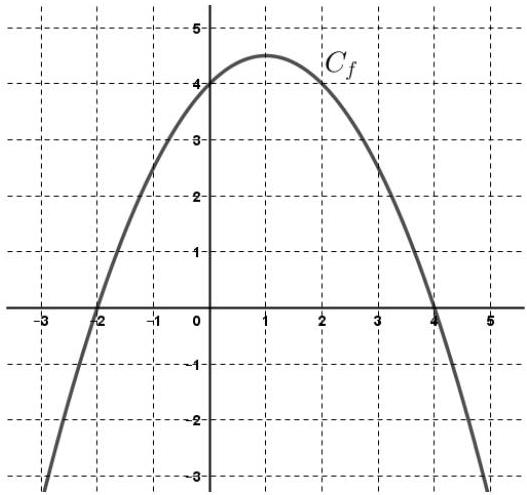
\includegraphics[scale=0.42]{Img01}
\end{minipage}
\vspace*{-0.7cm}
\exerciceDS{}
\begin{minipage}[c]{0.48\linewidth}
	On donne ci-contre la courbe représentative d'une fonction $f$ définie sur $[-3,5 ; 4,8]$. Répondre aux questions suivantes en utilisant ce graphique.

\begin{enumMet}
  \item Donner la valeur de $f(0)$.
  \item Donner l'image de 3 par $f$.
  \item Quels sont les antécédents de -1 par $f$ ?
  \item Quelles sont les solutions de l'équation $f(x)=0$ ?
  \item Dresser le tableau de variation de $f$.
  \item Dresser le tableau de signe de $f$.\\

\end{enumMet}
\end{minipage} \hfill
\begin{minipage}[c]{0.48\linewidth}
	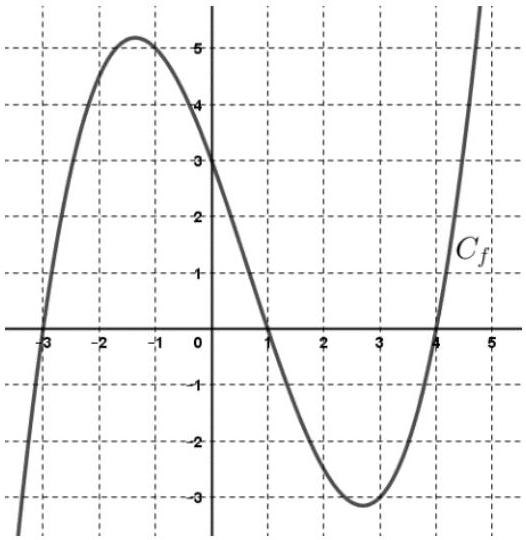
\includegraphics[scale=0.42]{Img02}
\end{minipage}
\vspace*{-0.7cm}
\exerciceDS{}
On considère le tableau de variation d'une fonction $g$ :

\begin{center}
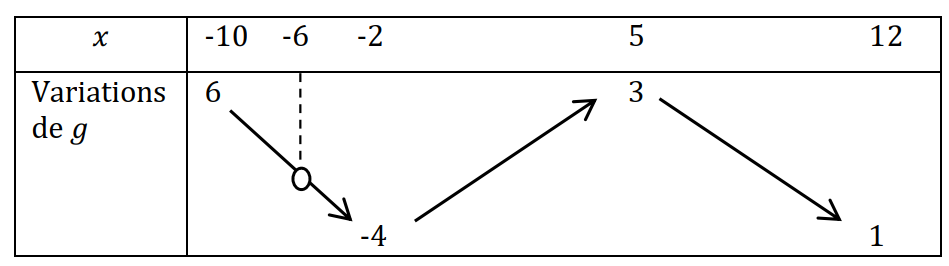
\includegraphics[scale=0.45]{Img03}
\end{center}

\begin{enumMet}
  \item Donner 3 exemples de nombres dont les images sont positives.
  \item On sait de plus que la fonction s'annule pour $x=-6$ et pour $x=1$. Dresser alors le tableau de signe de cette fonction.
\end{enumMet}

\section*{Capacité 8 : Equations de droites.}
\begin{brappel}
	\begin{itemMet}
		\item L' équation d' une droite non verticale est de la forme $y=m x+p$ ( $m$ étant appelé coefficient directeur, et $p$ ordonnée à l' origine).
		\item Lire graphiquement le coefficient directeur et l'ordonnée à l'origine d'une droite non verticale.
		\item Soit $d$ une droite non verticale d'équation $\mathrm{y}=m x+p$. Si $d$ passe par les points $\mathrm{A}\left(x_{A}, y_{A}\right)$ et $\mathrm{B}\left(x_{B}, y_{B}\right)$
		
		Alors, $m=\dfrac{y_{B}-y_{A}}{x_{B}-x_{A}}$
		\item L'équation d'une droite verticale est de la forme $x=k$.
	\end{itemMet}
\end{brappel}
\vspace*{-0.7cm}
\exerciceDS{}
\begin{minipage}[c]{0.45\linewidth}
	\begin{enumMet}
	\item Pour chacune des droites, compléter

	\begin{tabularx}{7.5cm}{|c|X|X|}
	\hline
	Droite & Coefficient & Ordonnée\\
	& directeur & à l'origine\\ \hline
	D1 &  &  \\
	\hline
	D2 &  &  \\
	\hline
	D3 &  &  \\
	\hline
	D4 &  &  \\
	\hline
	D5 &  &  \\
	\hline
	\end{tabularx}

	\item En déduire l'équation de chaque droite .\\
\end{enumMet}
\end{minipage} \hfill
\begin{minipage}[c]{0.52\linewidth}
	\begin{center}
		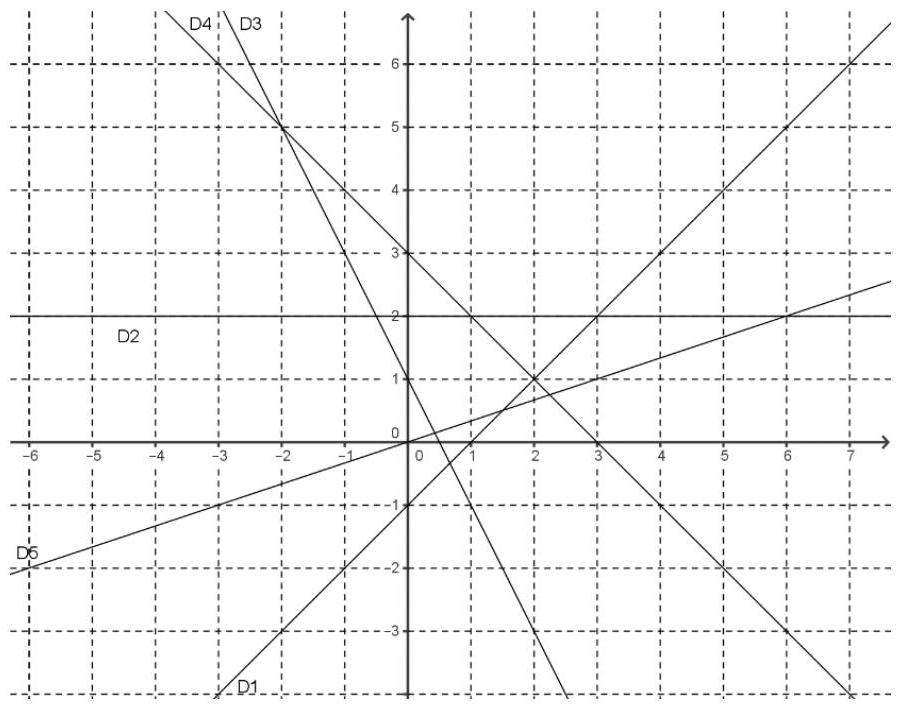
\includegraphics[scale=0.3]{Img04}
	\end{center}
\end{minipage}

\vspace*{-0.7cm}
\exerciceDS{}
Représenter dans un repère orthogonal :

\begin{enumMet}
  \item La droite $d_{1}$ d'équation $y=0,5 x+2$
  \item La droite $d_{2}$ passant par le point $A(3 ; 1)$ et d'ordonnée à l'origine 7
  \item La droite $d_{3}$ passant par le points $B(2 ;-2)$ et de coefficient directeur -1 .
  \item La droite $d_{4}$ d'équation: $y=-3 x$.
  \item La droite $d_{5}$ passant par $\mathrm{D}(1 ; 2)$ et de coefficient directeur 0 .
  \item La droite $d_{6}$ d'équation: $y=-\dfrac{1}{3} x+2$
  \item La droite $d_{7}$ d'équation: $x=-5$.
\end{enumMet}
\vspace*{-0.8cm}
\exerciceDS{}
\begin{enumMet}
  \item On désire déterminer l'équation de la droite passant par les points $A(5 ; 6)$ et $B(7 ;-2)$.
\begin{enumMet}
	\item Déterminer, par le calcul, le coefficient directeur $m$ de la droite.
	\item L'équation de la droite (AB) est alors de la forme $y=\cdots \cdot x+p$.
	\item Remplacer $x$ et $y$ par les coordonnées de $A$. En déduire la valeur de $p$.
	\item Déterminer alors l'équation de la droite (AB).
\end{enumMet}
  \item Déterminer l'équation de la droite passant par les points $M(-5 ;-14)$ et $N(1 ; 4)$.
  \item Le point $\mathrm{R}(10,31)$ appartient-il à une de ces deux droites ?
\end{enumMet}

\section*{Capacité 9 : Etudier le signe d'une fonction.}
\begin{brappel}
	\grasInProp{Méthode :}
	\begin{itemMet}
		\item Fonctions affines : voir cours seconde.
		\item Autres fonctions : se ramener à un produit ou à un quotient de fonctions.
	\end{itemMet}
\end{brappel}
\vspace*{-0.7cm}
\exerciceDS{}
Dresser le tableau de signe des fonctions suivantes :

\begin{multicols}{3}
	\begin{enumMet}
	\item $f(x)=(2 x+1)(x-3)$
	\item $g(x)=-2 x+3$
	\item $h(x)=x+5$
	\item $j(x)=(-2 x+6)(3+x)$
	\item $k(x)=4 x^{2}-3 x$
	\item $l(x)=\dfrac{2 x+1}{2-x}$
	\item $m(x)=\dfrac{1-3 x}{-1-x}$
	\item $n(x)=1-\dfrac{1}{x}$
\end{enumMet}
\end{multicols}

\section*{Capacité 10 : Les vecteurs.}
\begin{brappel}
	\begin{itemMet}
		\item Lire les coordonnées d'un vecteur.
		\item Savoir calculer les coordonnées d'un vecteur.
		
		Considérons les points $\mathrm{A}\left(x_{A} ; y_{A}\right)$ et $\mathrm{B}\left(x_{B} ; y_{B}\right)$. Les coordonnées du vecteur $\vv{A B}$ sont $\CoordSV{x_{B}-x_{A}}{y_{B}-y_{A}}$
		\item Relation de Chasles: Soient $\mathrm{A}, \mathrm{B}$ et C trois points du plan : $\vv{A B}+\vv{B C}=\vv{A C}$
		\item Déterminant de deux vecteurs. On considère les vecteurs $\Coord{u}{x}{y}$ et $\Coord{v}{x'}{y'}$. Alors :
		
		$\operatorname{det}(\vv{u} ; \vv{v})=\left|\begin{array}{ll}x & x' \\ y & y'\end{array}\right|=x y'-y x'$.
		\item Colinéarité de deux vecteurs.
		
		Deux vecteurs sont colinéaires si et seulement si leur déterminant est nul.
	\end{itemMet}
\end{brappel}

\vspace*{-0.7cm}
\exerciceDS{}
les questions 1,2 et 3 sont indépendantes

\begin{enumMet}
  \item Lire, dans le repère ci-contre, les coordonnées des vecteurs représentés :
  \begin{center}
  	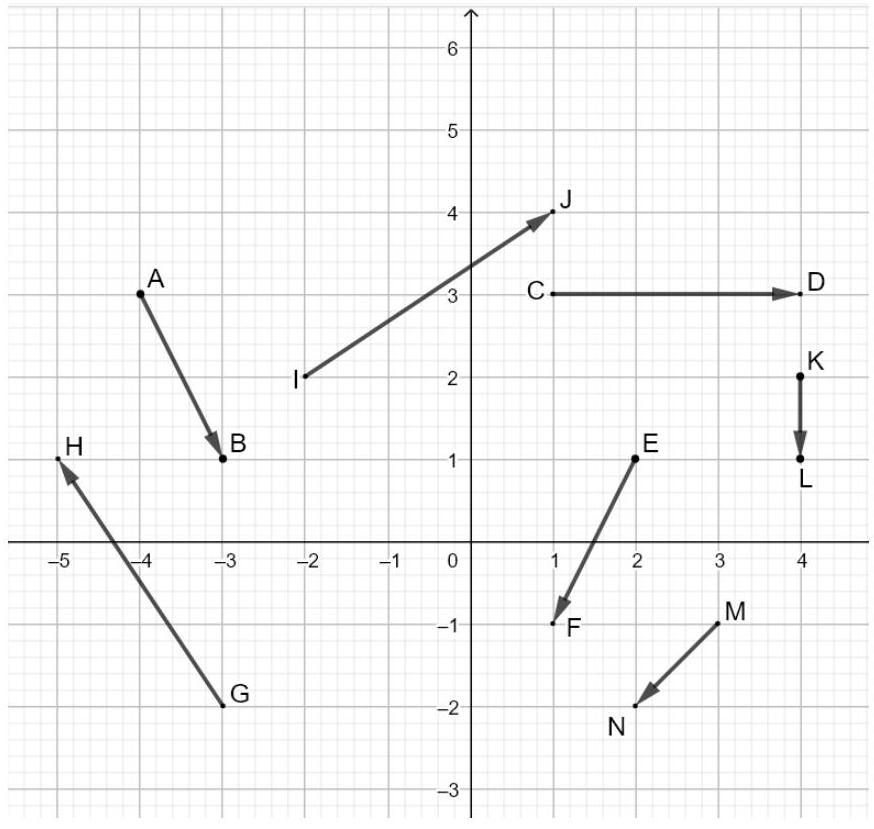
\includegraphics[scale=0.28]{Img05}
  \end{center}

  \item Dans un repère, on considère les points $\mathrm{A}(2 ; 1) ; \mathrm{B}(3 ;-4)$ et $\mathrm{C}(2 ; 0)$. On veut placer un point $\mathrm{M}(x ; y)$ tel que : $\vv{A M}=\vv{A B}+\vv{A C}$.
	\begin{enumMet}
		\item Calculer les coordonnées des vecteurs $\vv{A B}$ et $\vv{A C}$.
		\item Calculer les coordonnées de $\vv{A B}+\vv{A C}$.
		\item Exprimer les coordonnées du vecteur $\vv{A M}$ en fonction de $x$ et de $y$.
		\item Déterminer alors les coordonnées de M.
	\end{enumMet}
  \item Dans un repère, on considère les points $\mathrm{A}(3 ;-1) ; \mathrm{B}(0 ; 5)$ et $\mathrm{C}(-4 ; 1)$.
  
  On veut placer un point $\mathrm{M}(x ; y)$ tel que $: \vv{B M}=2 \vv{B C}-\vv{A B}$.
  \begin{enumMet}
  	\item Calculer les coordonnées de $2 \vv{B C}-\vv{A B}$.
	\item Exprimer les coordonnées du vecteur $\vv{B M}$ en fonction de $x$ et de $y$.
	\item Déterminer alors les coordonnées de M.
  \end{enumMet}
\end{enumMet}

\vspace*{-0.8cm}
\exerciceDS{}
Simplifier, au maximum, les expressions suivantes en utilisant la relation de Chasles:\\
Soient $\mathrm{R}, \mathrm{S}, \mathrm{T}, \mathrm{U}$ et V des points du plan.
\begin{multicols}{3}
	\begin{enumMet}
	\item $\vv{R T}+\vv{T U}$
	\item $\vv{T U}+\vv{U S}$
	\item $\vv{T U}+\vv{V T}$
	\item $\vv{T U}-\vv{T U}$
	\item $\vv{T U}+\vv{U S}+\vv{S R}$
\end{enumMet}
\end{multicols}
\vspace*{-0.8cm}
\exerciceDS{}
les questions 1,2, 3,4 et 5 sont indépendantes.

\begin{enumMet}
  \item Dire si les vecteurs suivants sont (ou ne sont pas) colinéaires.
	\begin{multicols}{2}
		\begin{enumMet}
		\item $\Coord{u}{2}{9}$ et $\Coord{v}{-6}{-27}$.
		\item $\Coord{u}{4}{-2}$ et $\Coord{v}{6}{3}$.
	\end{enumMet}
	\end{multicols}
  \item On considère les points suivants : $\mathrm{R}(-4 ; 1) ; \mathrm{S}(3 ;-2) ; \mathrm{T}(5 ; 7)$ et $U(13,4 ; 3,4)$.
  
  Les droites (RS) et (TU) sont-elles parallèles ?
  \item On considère les points suivants : $\mathrm{R}(-4 ; 1) ; \mathrm{S}(-1 ;-2) ; \mathrm{T}(5 ;-5)$.
  
  Les points $\mathrm{R}, \mathrm{S}$ et T sont-ils alignés ?
  \item On considère les vecteurs $\Coord{u}{2}{9}$ et $\Coord{v}{-6}{z}$. Pour quelle valeur du réel z ; ces deux vecteurs sont-ils colinéaires?
  \item On considère les points suivants : $\mathrm{R}(-4 ; 1) ; \mathrm{S}(-1 ;-2) ; \mathrm{T}(w ;-5)$. Pour quelle valeur du réel $w$, ces points sont-ils alignés ?
\end{enumMet}
\end{document}